\begin{frame}{Recognizing Conversational Roles}
  \centering
    \begin{columns}[T] % align columns
      \begin{column}{.5\textwidth}
        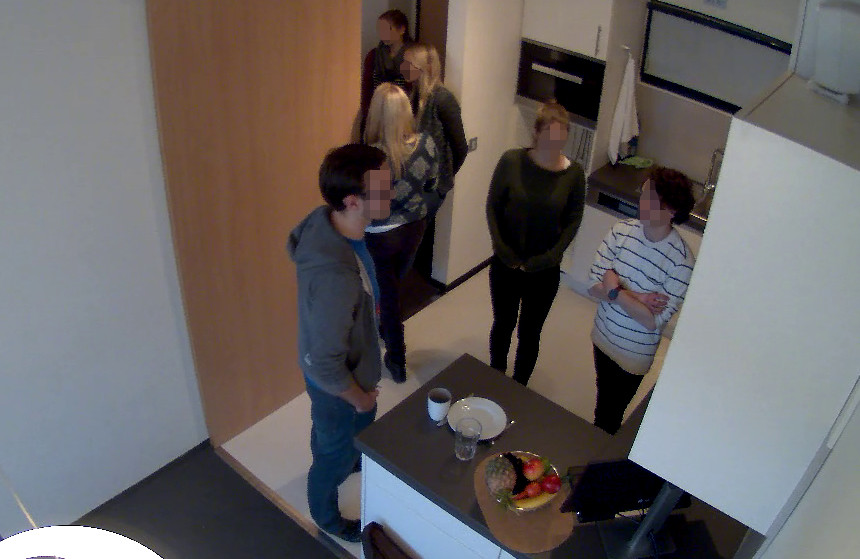
\includegraphics[trim={4.1cm 0 0 0},clip,width=\textwidth]{conversational_group}
      \end{column}
      \begin{column}{.5\textwidth}
        \vspace{10pt}
        \textbf{RQ4: Conversational Roles}\\\vspace{5pt} 
        \onslide<2->{In \textcolor{myblue}{unconstrained interactions} in a smart environment: } \onslide<3->{How can the \textcolor{myblue}{conversational role} of an \textcolor{myblue}{agent} be recognized?}\\
      \vspace{10pt}
       \onslide<4->\(\rightarrow\) \hspace{5pt} Simple Models\\
       \vspace{5pt}
       \onslide<5->\(\rightarrow\) \hspace{5pt} Low-Level Features\\
       \vspace{5pt}
       \onslide<6->\(\rightarrow\) \hspace{5pt} Time Sequences\\
      \end{column}
    \end{columns}
  \pnote{14-5}
\end{frame}
\begin{frame}{Demonstration Corpus}
  \begin{columns}[T] % align columns
    \begin{column}{.5\textwidth}
      \centering
      \onslide<1->{\resizebox{\textwidth}{!}{%
        \def\svgwidth{1.5\textwidth}
        \input{generated/csra_map_annotations.pdf_tex}
      }}
    \end{column}%
    \begin{column}{.5\textwidth}
      \resizebox{\textwidth}{!}{%
        \scriptsize
        \begin{tikzpicture}
        \action<1->{\node (c) at (0,0)
        {
          \resizebox{\textwidth}{!}{%
          \def\svgwidth{\textwidth}
          \input{generated/defence_role_annotations_real-image.pdf_tex}
          }
        };}
        \action<1->{\node (c) at (0,0)
        {
          \resizebox{\textwidth}{!}{%
          \def\svgwidth{\textwidth}
          \input{generated/defence_role_annotations_real-groups.pdf_tex}
          }
        };}
        \action<2->{\node (c) at (0,0)
        {
          \resizebox{\textwidth}{!}{%
          \def\svgwidth{\textwidth}
          \input{generated/defence_role_annotations_real-speaker.pdf_tex}
          }
        };}
         \action<3->{\node (c) at (0,0)
        {
          \resizebox{\textwidth}{!}{%
          \def\svgwidth{\textwidth}
          \input{generated/defence_role_annotations_real-addressee.pdf_tex}
          }
        };}
         \action<4->{\node (c) at (0,0)
        {
          \resizebox{\textwidth}{!}{%
          \def\svgwidth{\textwidth}
          \input{generated/defence_role_annotations_real-sideparticipant.pdf_tex}
          }
        };}
         \end{tikzpicture}
      }
    \end{column}%
  \end{columns}
        57 Minutes of 2 Agents at \SI{15}{\Hz} \(\rightarrow\) \SI{102}{\kilo\nothing} Observations \\
        \footnotesize
        \onslide<2-> \textcolor{myred}{Speaker} (3408) 
        \onslide<3-> \textcolor{mygreen}{Addressee} (5689)
        \onslide<4-> \textcolor{myblue}{Side-Participant} (18358)
        \onslide<5-> \textcolor{black}{Non-Participant} (74213)
  \pnote{14-5}
\end{frame}
\begin{frame}{Simple Models \& High-Level Features}
  \centering
  \resizebox{.8\textwidth}{!}{%
    \begin{tikzpicture}
    \action<1->{\node (c) at (0,0)
    {
      \resizebox{.7\textwidth}{!}{%
      \def\svgwidth{0.98\textwidth}
         {\footnotesize
         \input{generated/rule-model-defence.pdf_tex}
         }
      }
    };}
    \action<2->{\node (c) at (0,-90pt)
    {
      \resizebox{.6\textwidth}{!}{%
      \def\svgwidth{0.98\textwidth}
         {\footnotesize
         \input{generated/bn-role-defence.pdf_tex}
         }
      }
    };}
     \end{tikzpicture}
  }
  \pnote{14-5}
\end{frame}
\begin{frame}{Low-Level Features \& Time Sequences}
      \centering
      \vspace{20pt}
      \resizebox{.8\textwidth}{!}{%
          \scriptsize
          \begin{tikzpicture}
          \node (b) at (0,0)
          {
            \resizebox{1.35\textwidth}{!}{%
            \def\svgwidth{.3\textwidth}
            \input{generated/nnl-defence-dense.pdf_tex}
            }
          };
          \action<1->{\node (c) at (30,0)
          {
            \resizebox{1.35\textwidth}{!}{%
            \def\svgwidth{.3\textwidth}
            \input{generated/nnl-defence-t2.pdf_tex}
            }
          };}
          \action<1->{\node (c) at (30,0)
          {
            \resizebox{1.35\textwidth}{!}{%
            \def\svgwidth{.3\textwidth}
            \input{generated/nnl-defence-t1.pdf_tex}
            }
          };}
          \action<1->{\node (c) at (30,0)
          {
            \resizebox{1.35\textwidth}{!}{%
            \def\svgwidth{.3\textwidth}
            \input{generated/nnl-defence-lstm.pdf_tex}
            }
          };}
           \end{tikzpicture}
        }
        \begin{itemize}[label=-]
          \item<2-> Train with different feature sets, number of layers, units in each layer
          \item<3-> Feature sets: High-level (4D as Bayes Model) \(\rightarrow\) Low-Level (148D)
          \item<4-> For lstm: sequences of 15 observations \(\approx\) \SI{1}{\second}
        \end{itemize}
  \pnote{14-5}
\end{frame}
\begin{frame}{Results - Confusion Matrices}
  \begin{columns}[T] % align columns
    \begin{column}{.65\textwidth}
      \resizebox{1.\textwidth}{!}{%
        \scriptsize
        \begin{tikzpicture}
          \action<3->{\node (b) at (0,0)
          {
            \resizebox{\textwidth}{!}{%
              % Created by tikzDevice version 0.12
% !TEX encoding = UTF-8 Unicode
\begin{tikzpicture}[x=1pt,y=1pt]
\definecolor{fillColor}{RGB}{255,255,255}
\path[use as bounding box,fill=fillColor,fill opacity=0.00] (0,0) rectangle (398.34,246.17);
\begin{scope}
\path[clip] (  0.00,  0.00) rectangle (398.34,246.17);
\definecolor{drawColor}{RGB}{255,255,255}
\definecolor{fillColor}{gray}{0.98}

\path[draw=drawColor,line width= 0.6pt,line join=round,line cap=round,fill=fillColor] (  0.00,  0.00) rectangle (398.34,246.17);
\end{scope}
\begin{scope}
\path[clip] (100.50,152.22) rectangle (243.92,223.87);
\definecolor{drawColor}{RGB}{255,255,255}

\path[draw=drawColor,line width= 0.6pt,line join=round] (100.50,162.46) --
	(243.92,162.46);

\path[draw=drawColor,line width= 0.6pt,line join=round] (100.50,179.51) --
	(243.92,179.51);

\path[draw=drawColor,line width= 0.6pt,line join=round] (100.50,196.57) --
	(243.92,196.57);

\path[draw=drawColor,line width= 0.6pt,line join=round] (100.50,213.63) --
	(243.92,213.63);

\path[draw=drawColor,line width= 0.6pt,line join=round] (120.98,152.22) --
	(120.98,223.87);

\path[draw=drawColor,line width= 0.6pt,line join=round] (155.13,152.22) --
	(155.13,223.87);

\path[draw=drawColor,line width= 0.6pt,line join=round] (189.28,152.22) --
	(189.28,223.87);

\path[draw=drawColor,line width= 0.6pt,line join=round] (223.43,152.22) --
	(223.43,223.87);
\definecolor{fillColor}{RGB}{77,175,74}

\path[fill=fillColor,fill opacity=0.39] (103.91,205.10) rectangle (138.06,222.16);
\definecolor{fillColor}{RGB}{228,26,28}

\path[fill=fillColor,fill opacity=0.47] (138.06,205.10) rectangle (172.21,222.16);
\definecolor{fillColor}{RGB}{228,26,28}

\path[fill=fillColor,fill opacity=0.31] (172.21,205.10) rectangle (206.35,222.16);
\definecolor{fillColor}{RGB}{228,26,28}

\path[fill=fillColor,fill opacity=0.16] (206.35,205.10) rectangle (240.50,222.16);
\definecolor{fillColor}{RGB}{228,26,28}

\path[fill=fillColor,fill opacity=0.13] (103.91,188.04) rectangle (138.06,205.10);
\definecolor{fillColor}{RGB}{77,175,74}

\path[fill=fillColor,fill opacity=0.75] (138.06,188.04) rectangle (172.21,205.10);
\definecolor{fillColor}{RGB}{228,26,28}

\path[fill=fillColor,fill opacity=0.27] (172.21,188.04) rectangle (206.35,205.10);
\definecolor{fillColor}{RGB}{228,26,28}

\path[fill=fillColor,fill opacity=0.17] (206.35,188.04) rectangle (240.50,205.10);
\definecolor{fillColor}{RGB}{228,26,28}

\path[fill=fillColor,fill opacity=0.11] (103.91,170.99) rectangle (138.06,188.04);
\definecolor{fillColor}{RGB}{228,26,28}

\path[fill=fillColor,fill opacity=0.45] (138.06,170.99) rectangle (172.21,188.04);
\definecolor{fillColor}{RGB}{77,175,74}

\path[fill=fillColor,fill opacity=0.51] (172.21,170.99) rectangle (206.35,188.04);
\definecolor{fillColor}{RGB}{228,26,28}

\path[fill=fillColor,fill opacity=0.25] (206.35,170.99) rectangle (240.50,188.04);
\definecolor{fillColor}{RGB}{228,26,28}

\path[fill=fillColor,fill opacity=0.10] (103.91,153.93) rectangle (138.06,170.99);
\definecolor{fillColor}{RGB}{228,26,28}

\path[fill=fillColor,fill opacity=0.11] (138.06,153.93) rectangle (172.21,170.99);
\definecolor{fillColor}{RGB}{228,26,28}

\path[fill=fillColor,fill opacity=0.16] (172.21,153.93) rectangle (206.35,170.99);
\definecolor{fillColor}{RGB}{77,175,74}

\path[fill=fillColor,fill opacity=0.96] (206.35,153.93) rectangle (240.50,170.99);
\definecolor{drawColor}{RGB}{0,0,0}

\node[text=drawColor,anchor=base,inner sep=0pt, outer sep=0pt, scale=  1.14] at (120.98,209.71) {0.32};

\node[text=drawColor,anchor=base,inner sep=0pt, outer sep=0pt, scale=  1.14] at (155.13,209.71) {0.40};

\node[text=drawColor,anchor=base,inner sep=0pt, outer sep=0pt, scale=  1.14] at (189.28,209.71) {0.23};

\node[text=drawColor,anchor=base,inner sep=0pt, outer sep=0pt, scale=  1.14] at (223.43,209.71) {0.06};

\node[text=drawColor,anchor=base,inner sep=0pt, outer sep=0pt, scale=  1.14] at (120.98,192.66) {0.03};

\node[text=drawColor,anchor=base,inner sep=0pt, outer sep=0pt, scale=  1.14] at (155.13,192.66) {0.70};

\node[text=drawColor,anchor=base,inner sep=0pt, outer sep=0pt, scale=  1.14] at (189.28,192.66) {0.19};

\node[text=drawColor,anchor=base,inner sep=0pt, outer sep=0pt, scale=  1.14] at (223.43,192.66) {0.08};

\node[text=drawColor,anchor=base,inner sep=0pt, outer sep=0pt, scale=  1.14] at (120.98,175.60) {0.01};

\node[text=drawColor,anchor=base,inner sep=0pt, outer sep=0pt, scale=  1.14] at (155.13,175.60) {0.38};

\node[text=drawColor,anchor=base,inner sep=0pt, outer sep=0pt, scale=  1.14] at (189.28,175.60) {0.45};

\node[text=drawColor,anchor=base,inner sep=0pt, outer sep=0pt, scale=  1.14] at (223.43,175.60) {0.17};

\node[text=drawColor,anchor=base,inner sep=0pt, outer sep=0pt, scale=  1.14] at (120.98,158.54) {0.00};

\node[text=drawColor,anchor=base,inner sep=0pt, outer sep=0pt, scale=  1.14] at (155.13,158.54) {0.01};

\node[text=drawColor,anchor=base,inner sep=0pt, outer sep=0pt, scale=  1.14] at (189.28,158.54) {0.06};

\node[text=drawColor,anchor=base,inner sep=0pt, outer sep=0pt, scale=  1.14] at (223.43,158.54) {0.93};
\end{scope}
\begin{scope}
\path[clip] (100.50, 58.27) rectangle (243.92,129.92);
\definecolor{drawColor}{RGB}{255,255,255}

\path[draw=drawColor,line width= 0.6pt,line join=round] (100.50, 68.50) --
	(243.92, 68.50);

\path[draw=drawColor,line width= 0.6pt,line join=round] (100.50, 85.56) --
	(243.92, 85.56);

\path[draw=drawColor,line width= 0.6pt,line join=round] (100.50,102.62) --
	(243.92,102.62);

\path[draw=drawColor,line width= 0.6pt,line join=round] (100.50,119.68) --
	(243.92,119.68);

\path[draw=drawColor,line width= 0.6pt,line join=round] (120.98, 58.27) --
	(120.98,129.92);

\path[draw=drawColor,line width= 0.6pt,line join=round] (155.13, 58.27) --
	(155.13,129.92);

\path[draw=drawColor,line width= 0.6pt,line join=round] (189.28, 58.27) --
	(189.28,129.92);

\path[draw=drawColor,line width= 0.6pt,line join=round] (223.43, 58.27) --
	(223.43,129.92);
\definecolor{fillColor}{RGB}{77,175,74}

\path[fill=fillColor,fill opacity=0.39] (103.91,111.15) rectangle (138.06,128.21);
\definecolor{fillColor}{RGB}{228,26,28}

\path[fill=fillColor,fill opacity=0.20] (138.06,111.15) rectangle (172.21,128.21);
\definecolor{fillColor}{RGB}{228,26,28}

\path[fill=fillColor,fill opacity=0.55] (172.21,111.15) rectangle (206.35,128.21);
\definecolor{fillColor}{RGB}{228,26,28}

\path[fill=fillColor,fill opacity=0.18] (206.35,111.15) rectangle (240.50,128.21);
\definecolor{fillColor}{RGB}{228,26,28}

\path[fill=fillColor,fill opacity=0.14] (103.91, 94.09) rectangle (138.06,111.15);
\definecolor{fillColor}{RGB}{77,175,74}

\path[fill=fillColor,fill opacity=0.25] (138.06, 94.09) rectangle (172.21,111.15);
\definecolor{fillColor}{RGB}{228,26,28}

\path[fill=fillColor,fill opacity=0.82] (172.21, 94.09) rectangle (206.35,111.15);
\definecolor{fillColor}{RGB}{228,26,28}

\path[fill=fillColor,fill opacity=0.12] (206.35, 94.09) rectangle (240.50,111.15);
\definecolor{fillColor}{RGB}{228,26,28}

\path[fill=fillColor,fill opacity=0.12] (103.91, 77.03) rectangle (138.06, 94.09);
\definecolor{fillColor}{RGB}{228,26,28}

\path[fill=fillColor,fill opacity=0.16] (138.06, 77.03) rectangle (172.21, 94.09);
\definecolor{fillColor}{RGB}{77,175,74}

\path[fill=fillColor,fill opacity=0.76] (172.21, 77.03) rectangle (206.35, 94.09);
\definecolor{fillColor}{RGB}{228,26,28}

\path[fill=fillColor,fill opacity=0.29] (206.35, 77.03) rectangle (240.50, 94.09);
\definecolor{fillColor}{RGB}{228,26,28}

\path[fill=fillColor,fill opacity=0.10] (103.91, 59.97) rectangle (138.06, 77.03);

\path[fill=fillColor,fill opacity=0.10] (138.06, 59.97) rectangle (172.21, 77.03);
\definecolor{fillColor}{RGB}{228,26,28}

\path[fill=fillColor,fill opacity=0.13] (172.21, 59.97) rectangle (206.35, 77.03);
\definecolor{fillColor}{RGB}{77,175,74}

\path[fill=fillColor] (206.35, 59.97) rectangle (240.50, 77.03);
\definecolor{drawColor}{RGB}{0,0,0}

\node[text=drawColor,anchor=base,inner sep=0pt, outer sep=0pt, scale=  1.14] at (120.98,115.76) {0.32};

\node[text=drawColor,anchor=base,inner sep=0pt, outer sep=0pt, scale=  1.14] at (155.13,115.76) {0.11};

\node[text=drawColor,anchor=base,inner sep=0pt, outer sep=0pt, scale=  1.14] at (189.28,115.76) {0.48};

\node[text=drawColor,anchor=base,inner sep=0pt, outer sep=0pt, scale=  1.14] at (223.43,115.76) {0.09};

\node[text=drawColor,anchor=base,inner sep=0pt, outer sep=0pt, scale=  1.14] at (120.98, 98.70) {0.04};

\node[text=drawColor,anchor=base,inner sep=0pt, outer sep=0pt, scale=  1.14] at (155.13, 98.70) {0.16};

\node[text=drawColor,anchor=base,inner sep=0pt, outer sep=0pt, scale=  1.14] at (189.28, 98.70) {0.78};

\node[text=drawColor,anchor=base,inner sep=0pt, outer sep=0pt, scale=  1.14] at (223.43, 98.70) {0.02};

\node[text=drawColor,anchor=base,inner sep=0pt, outer sep=0pt, scale=  1.14] at (120.98, 81.64) {0.02};

\node[text=drawColor,anchor=base,inner sep=0pt, outer sep=0pt, scale=  1.14] at (155.13, 81.64) {0.07};

\node[text=drawColor,anchor=base,inner sep=0pt, outer sep=0pt, scale=  1.14] at (189.28, 81.64) {0.71};

\node[text=drawColor,anchor=base,inner sep=0pt, outer sep=0pt, scale=  1.14] at (223.43, 81.64) {0.21};

\node[text=drawColor,anchor=base,inner sep=0pt, outer sep=0pt, scale=  1.14] at (120.98, 64.58) {0.00};

\node[text=drawColor,anchor=base,inner sep=0pt, outer sep=0pt, scale=  1.14] at (155.13, 64.58) {0.00};

\node[text=drawColor,anchor=base,inner sep=0pt, outer sep=0pt, scale=  1.14] at (189.28, 64.58) {0.03};

\node[text=drawColor,anchor=base,inner sep=0pt, outer sep=0pt, scale=  1.14] at (223.43, 64.58) {0.97};
\end{scope}
\begin{scope}
\path[clip] (249.42,152.22) rectangle (392.84,223.87);
\definecolor{drawColor}{RGB}{255,255,255}

\path[draw=drawColor,line width= 0.6pt,line join=round] (249.42,162.46) --
	(392.84,162.46);

\path[draw=drawColor,line width= 0.6pt,line join=round] (249.42,179.51) --
	(392.84,179.51);

\path[draw=drawColor,line width= 0.6pt,line join=round] (249.42,196.57) --
	(392.84,196.57);

\path[draw=drawColor,line width= 0.6pt,line join=round] (249.42,213.63) --
	(392.84,213.63);

\path[draw=drawColor,line width= 0.6pt,line join=round] (269.91,152.22) --
	(269.91,223.87);

\path[draw=drawColor,line width= 0.6pt,line join=round] (304.05,152.22) --
	(304.05,223.87);

\path[draw=drawColor,line width= 0.6pt,line join=round] (338.20,152.22) --
	(338.20,223.87);

\path[draw=drawColor,line width= 0.6pt,line join=round] (372.35,152.22) --
	(372.35,223.87);
\definecolor{fillColor}{RGB}{77,175,74}

\path[fill=fillColor,fill opacity=0.41] (252.83,205.10) rectangle (286.98,222.16);
\definecolor{fillColor}{RGB}{228,26,28}

\path[fill=fillColor,fill opacity=0.31] (286.98,205.10) rectangle (321.13,222.16);
\definecolor{fillColor}{RGB}{228,26,28}

\path[fill=fillColor,fill opacity=0.49] (321.13,205.10) rectangle (355.28,222.16);
\definecolor{fillColor}{RGB}{228,26,28}

\path[fill=fillColor,fill opacity=0.13] (355.28,205.10) rectangle (389.42,222.16);
\definecolor{fillColor}{RGB}{228,26,28}

\path[fill=fillColor,fill opacity=0.13] (252.83,188.04) rectangle (286.98,205.10);
\definecolor{fillColor}{RGB}{77,175,74}

\path[fill=fillColor,fill opacity=0.35] (286.98,188.04) rectangle (321.13,205.10);
\definecolor{fillColor}{RGB}{228,26,28}

\path[fill=fillColor,fill opacity=0.74] (321.13,188.04) rectangle (355.28,205.10);
\definecolor{fillColor}{RGB}{228,26,28}

\path[fill=fillColor,fill opacity=0.11] (355.28,188.04) rectangle (389.42,205.10);
\definecolor{fillColor}{RGB}{228,26,28}

\path[fill=fillColor,fill opacity=0.11] (252.83,170.99) rectangle (286.98,188.04);
\definecolor{fillColor}{RGB}{228,26,28}

\path[fill=fillColor,fill opacity=0.20] (286.98,170.99) rectangle (321.13,188.04);
\definecolor{fillColor}{RGB}{77,175,74}

\path[fill=fillColor,fill opacity=0.84] (321.13,170.99) rectangle (355.28,188.04);
\definecolor{fillColor}{RGB}{228,26,28}

\path[fill=fillColor,fill opacity=0.19] (355.28,170.99) rectangle (389.42,188.04);
\definecolor{fillColor}{RGB}{228,26,28}

\path[fill=fillColor,fill opacity=0.10] (252.83,153.93) rectangle (286.98,170.99);

\path[fill=fillColor,fill opacity=0.10] (286.98,153.93) rectangle (321.13,170.99);
\definecolor{fillColor}{RGB}{228,26,28}

\path[fill=fillColor,fill opacity=0.17] (321.13,153.93) rectangle (355.28,170.99);
\definecolor{fillColor}{RGB}{77,175,74}

\path[fill=fillColor,fill opacity=0.95] (355.28,153.93) rectangle (389.42,170.99);
\definecolor{drawColor}{RGB}{0,0,0}

\node[text=drawColor,anchor=base,inner sep=0pt, outer sep=0pt, scale=  1.14] at (269.91,209.71) {0.33};

\node[text=drawColor,anchor=base,inner sep=0pt, outer sep=0pt, scale=  1.14] at (304.05,209.71) {0.22};

\node[text=drawColor,anchor=base,inner sep=0pt, outer sep=0pt, scale=  1.14] at (338.20,209.71) {0.42};

\node[text=drawColor,anchor=base,inner sep=0pt, outer sep=0pt, scale=  1.14] at (372.35,209.71) {0.03};

\node[text=drawColor,anchor=base,inner sep=0pt, outer sep=0pt, scale=  1.14] at (269.91,192.66) {0.03};

\node[text=drawColor,anchor=base,inner sep=0pt, outer sep=0pt, scale=  1.14] at (304.05,192.66) {0.27};

\node[text=drawColor,anchor=base,inner sep=0pt, outer sep=0pt, scale=  1.14] at (338.20,192.66) {0.69};

\node[text=drawColor,anchor=base,inner sep=0pt, outer sep=0pt, scale=  1.14] at (372.35,192.66) {0.01};

\node[text=drawColor,anchor=base,inner sep=0pt, outer sep=0pt, scale=  1.14] at (269.91,175.60) {0.01};

\node[text=drawColor,anchor=base,inner sep=0pt, outer sep=0pt, scale=  1.14] at (304.05,175.60) {0.11};

\node[text=drawColor,anchor=base,inner sep=0pt, outer sep=0pt, scale=  1.14] at (338.20,175.60) {0.79};

\node[text=drawColor,anchor=base,inner sep=0pt, outer sep=0pt, scale=  1.14] at (372.35,175.60) {0.09};

\node[text=drawColor,anchor=base,inner sep=0pt, outer sep=0pt, scale=  1.14] at (269.91,158.54) {0.00};

\node[text=drawColor,anchor=base,inner sep=0pt, outer sep=0pt, scale=  1.14] at (304.05,158.54) {0.00};

\node[text=drawColor,anchor=base,inner sep=0pt, outer sep=0pt, scale=  1.14] at (338.20,158.54) {0.08};

\node[text=drawColor,anchor=base,inner sep=0pt, outer sep=0pt, scale=  1.14] at (372.35,158.54) {0.92};
\end{scope}
\begin{scope}
\path[clip] (249.42, 58.27) rectangle (392.84,129.92);
\definecolor{drawColor}{RGB}{255,255,255}

\path[draw=drawColor,line width= 0.6pt,line join=round] (249.42, 68.50) --
	(392.84, 68.50);

\path[draw=drawColor,line width= 0.6pt,line join=round] (249.42, 85.56) --
	(392.84, 85.56);

\path[draw=drawColor,line width= 0.6pt,line join=round] (249.42,102.62) --
	(392.84,102.62);

\path[draw=drawColor,line width= 0.6pt,line join=round] (249.42,119.68) --
	(392.84,119.68);

\path[draw=drawColor,line width= 0.6pt,line join=round] (269.91, 58.27) --
	(269.91,129.92);

\path[draw=drawColor,line width= 0.6pt,line join=round] (304.05, 58.27) --
	(304.05,129.92);

\path[draw=drawColor,line width= 0.6pt,line join=round] (338.20, 58.27) --
	(338.20,129.92);

\path[draw=drawColor,line width= 0.6pt,line join=round] (372.35, 58.27) --
	(372.35,129.92);
\definecolor{fillColor}{RGB}{77,175,74}

\path[fill=fillColor,fill opacity=0.45] (252.83,111.15) rectangle (286.98,128.21);
\definecolor{fillColor}{RGB}{228,26,28}

\path[fill=fillColor,fill opacity=0.23] (286.98,111.15) rectangle (321.13,128.21);
\definecolor{fillColor}{RGB}{228,26,28}

\path[fill=fillColor,fill opacity=0.54] (321.13,111.15) rectangle (355.28,128.21);
\definecolor{fillColor}{RGB}{228,26,28}

\path[fill=fillColor,fill opacity=0.12] (355.28,111.15) rectangle (389.42,128.21);
\definecolor{fillColor}{RGB}{228,26,28}

\path[fill=fillColor,fill opacity=0.15] (252.83, 94.09) rectangle (286.98,111.15);
\definecolor{fillColor}{RGB}{77,175,74}

\path[fill=fillColor,fill opacity=0.36] (286.98, 94.09) rectangle (321.13,111.15);
\definecolor{fillColor}{RGB}{228,26,28}

\path[fill=fillColor,fill opacity=0.71] (321.13, 94.09) rectangle (355.28,111.15);
\definecolor{fillColor}{RGB}{228,26,28}

\path[fill=fillColor,fill opacity=0.11] (355.28, 94.09) rectangle (389.42,111.15);
\definecolor{fillColor}{RGB}{228,26,28}

\path[fill=fillColor,fill opacity=0.12] (252.83, 77.03) rectangle (286.98, 94.09);
\definecolor{fillColor}{RGB}{228,26,28}

\path[fill=fillColor,fill opacity=0.16] (286.98, 77.03) rectangle (321.13, 94.09);
\definecolor{fillColor}{RGB}{77,175,74}

\path[fill=fillColor,fill opacity=0.80] (321.13, 77.03) rectangle (355.28, 94.09);
\definecolor{fillColor}{RGB}{228,26,28}

\path[fill=fillColor,fill opacity=0.24] (355.28, 77.03) rectangle (389.42, 94.09);
\definecolor{fillColor}{RGB}{228,26,28}

\path[fill=fillColor,fill opacity=0.10] (252.83, 59.97) rectangle (286.98, 77.03);

\path[fill=fillColor,fill opacity=0.10] (286.98, 59.97) rectangle (321.13, 77.03);
\definecolor{fillColor}{RGB}{228,26,28}

\path[fill=fillColor,fill opacity=0.14] (321.13, 59.97) rectangle (355.28, 77.03);
\definecolor{fillColor}{RGB}{77,175,74}

\path[fill=fillColor,fill opacity=0.98] (355.28, 59.97) rectangle (389.42, 77.03);
\definecolor{drawColor}{RGB}{0,0,0}

\node[text=drawColor,anchor=base,inner sep=0pt, outer sep=0pt, scale=  1.14] at (269.91,115.76) {0.37};

\node[text=drawColor,anchor=base,inner sep=0pt, outer sep=0pt, scale=  1.14] at (304.05,115.76) {0.14};

\node[text=drawColor,anchor=base,inner sep=0pt, outer sep=0pt, scale=  1.14] at (338.20,115.76) {0.47};

\node[text=drawColor,anchor=base,inner sep=0pt, outer sep=0pt, scale=  1.14] at (372.35,115.76) {0.02};

\node[text=drawColor,anchor=base,inner sep=0pt, outer sep=0pt, scale=  1.14] at (269.91, 98.70) {0.06};

\node[text=drawColor,anchor=base,inner sep=0pt, outer sep=0pt, scale=  1.14] at (304.05, 98.70) {0.28};

\node[text=drawColor,anchor=base,inner sep=0pt, outer sep=0pt, scale=  1.14] at (338.20, 98.70) {0.66};

\node[text=drawColor,anchor=base,inner sep=0pt, outer sep=0pt, scale=  1.14] at (372.35, 98.70) {0.01};

\node[text=drawColor,anchor=base,inner sep=0pt, outer sep=0pt, scale=  1.14] at (269.91, 81.64) {0.02};

\node[text=drawColor,anchor=base,inner sep=0pt, outer sep=0pt, scale=  1.14] at (304.05, 81.64) {0.07};

\node[text=drawColor,anchor=base,inner sep=0pt, outer sep=0pt, scale=  1.14] at (338.20, 81.64) {0.75};

\node[text=drawColor,anchor=base,inner sep=0pt, outer sep=0pt, scale=  1.14] at (372.35, 81.64) {0.15};

\node[text=drawColor,anchor=base,inner sep=0pt, outer sep=0pt, scale=  1.14] at (269.91, 64.58) {0.00};

\node[text=drawColor,anchor=base,inner sep=0pt, outer sep=0pt, scale=  1.14] at (304.05, 64.58) {0.00};

\node[text=drawColor,anchor=base,inner sep=0pt, outer sep=0pt, scale=  1.14] at (338.20, 64.58) {0.04};

\node[text=drawColor,anchor=base,inner sep=0pt, outer sep=0pt, scale=  1.14] at (372.35, 64.58) {0.95};
\end{scope}
\begin{scope}
\path[clip] (100.50,129.92) rectangle (243.92,146.72);
\definecolor{fillColor}{gray}{0.85}

\path[fill=fillColor] (100.50,129.92) rectangle (243.92,146.72);
\definecolor{drawColor}{gray}{0.10}

\node[text=drawColor,anchor=base,inner sep=0pt, outer sep=0pt, scale=  0.88] at (172.21,135.29) {Dense-Low-Level};
\end{scope}
\begin{scope}
\path[clip] (249.42,129.92) rectangle (392.84,146.72);
\definecolor{fillColor}{gray}{0.85}

\path[fill=fillColor] (249.42,129.92) rectangle (392.84,146.72);
\definecolor{drawColor}{gray}{0.10}

\node[text=drawColor,anchor=base,inner sep=0pt, outer sep=0pt, scale=  0.88] at (321.13,135.29) {Lstm-Rule};
\end{scope}
\begin{scope}
\path[clip] (100.50,223.87) rectangle (243.92,240.67);
\definecolor{fillColor}{gray}{0.85}

\path[fill=fillColor] (100.50,223.87) rectangle (243.92,240.67);
\definecolor{drawColor}{gray}{0.10}

\node[text=drawColor,anchor=base,inner sep=0pt, outer sep=0pt, scale=  0.88] at (172.21,229.24) {Rule};
\end{scope}
\begin{scope}
\path[clip] (249.42,223.87) rectangle (392.84,240.67);
\definecolor{fillColor}{gray}{0.85}

\path[fill=fillColor] (249.42,223.87) rectangle (392.84,240.67);
\definecolor{drawColor}{gray}{0.10}

\node[text=drawColor,anchor=base,inner sep=0pt, outer sep=0pt, scale=  0.88] at (321.13,229.24) {Bayes};
\end{scope}
\begin{scope}
\path[clip] (  0.00,  0.00) rectangle (398.34,246.17);
\definecolor{drawColor}{gray}{0.20}

\path[draw=drawColor,line width= 0.6pt,line join=round] (120.98, 55.52) --
	(120.98, 58.27);

\path[draw=drawColor,line width= 0.6pt,line join=round] (155.13, 55.52) --
	(155.13, 58.27);

\path[draw=drawColor,line width= 0.6pt,line join=round] (189.28, 55.52) --
	(189.28, 58.27);

\path[draw=drawColor,line width= 0.6pt,line join=round] (223.43, 55.52) --
	(223.43, 58.27);
\end{scope}
\begin{scope}
\path[clip] (  0.00,  0.00) rectangle (398.34,246.17);
\definecolor{drawColor}{RGB}{0,0,0}

\node[text=drawColor,rotate= 20.00,anchor=base east,inner sep=0pt, outer sep=0pt, scale=  1.10] at (123.58, 46.20) {Speaker};

\node[text=drawColor,rotate= 20.00,anchor=base east,inner sep=0pt, outer sep=0pt, scale=  1.10] at (157.72, 46.20) {Addressee};

\node[text=drawColor,rotate= 20.00,anchor=base east,inner sep=0pt, outer sep=0pt, scale=  1.10] at (191.87, 46.20) {Side-Participant};

\node[text=drawColor,rotate= 20.00,anchor=base east,inner sep=0pt, outer sep=0pt, scale=  1.10] at (226.02, 46.20) {Non-Participant};
\end{scope}
\begin{scope}
\path[clip] (  0.00,  0.00) rectangle (398.34,246.17);
\definecolor{drawColor}{gray}{0.20}

\path[draw=drawColor,line width= 0.6pt,line join=round] (269.91, 55.52) --
	(269.91, 58.27);

\path[draw=drawColor,line width= 0.6pt,line join=round] (304.05, 55.52) --
	(304.05, 58.27);

\path[draw=drawColor,line width= 0.6pt,line join=round] (338.20, 55.52) --
	(338.20, 58.27);

\path[draw=drawColor,line width= 0.6pt,line join=round] (372.35, 55.52) --
	(372.35, 58.27);
\end{scope}
\begin{scope}
\path[clip] (  0.00,  0.00) rectangle (398.34,246.17);
\definecolor{drawColor}{RGB}{0,0,0}

\node[text=drawColor,rotate= 20.00,anchor=base east,inner sep=0pt, outer sep=0pt, scale=  1.10] at (272.50, 46.20) {Speaker};

\node[text=drawColor,rotate= 20.00,anchor=base east,inner sep=0pt, outer sep=0pt, scale=  1.10] at (306.65, 46.20) {Addressee};

\node[text=drawColor,rotate= 20.00,anchor=base east,inner sep=0pt, outer sep=0pt, scale=  1.10] at (340.79, 46.20) {Side-Participant};

\node[text=drawColor,rotate= 20.00,anchor=base east,inner sep=0pt, outer sep=0pt, scale=  1.10] at (374.94, 46.20) {Non-Participant};
\end{scope}
\begin{scope}
\path[clip] (  0.00,  0.00) rectangle (398.34,246.17);
\definecolor{drawColor}{RGB}{0,0,0}

\node[text=drawColor,anchor=base east,inner sep=0pt, outer sep=0pt, scale=  1.10] at ( 95.55,158.67) {Non-Participant};

\node[text=drawColor,anchor=base east,inner sep=0pt, outer sep=0pt, scale=  1.10] at ( 95.55,175.73) {Side-Participant};

\node[text=drawColor,anchor=base east,inner sep=0pt, outer sep=0pt, scale=  1.10] at ( 95.55,192.79) {Addressee};

\node[text=drawColor,anchor=base east,inner sep=0pt, outer sep=0pt, scale=  1.10] at ( 95.55,209.85) {Speaker};
\end{scope}
\begin{scope}
\path[clip] (  0.00,  0.00) rectangle (398.34,246.17);
\definecolor{drawColor}{gray}{0.20}

\path[draw=drawColor,line width= 0.6pt,line join=round] ( 97.75,162.46) --
	(100.50,162.46);

\path[draw=drawColor,line width= 0.6pt,line join=round] ( 97.75,179.51) --
	(100.50,179.51);

\path[draw=drawColor,line width= 0.6pt,line join=round] ( 97.75,196.57) --
	(100.50,196.57);

\path[draw=drawColor,line width= 0.6pt,line join=round] ( 97.75,213.63) --
	(100.50,213.63);
\end{scope}
\begin{scope}
\path[clip] (  0.00,  0.00) rectangle (398.34,246.17);
\definecolor{drawColor}{RGB}{0,0,0}

\node[text=drawColor,anchor=base east,inner sep=0pt, outer sep=0pt, scale=  1.10] at ( 95.55, 64.71) {Non-Participant};

\node[text=drawColor,anchor=base east,inner sep=0pt, outer sep=0pt, scale=  1.10] at ( 95.55, 81.77) {Side-Participant};

\node[text=drawColor,anchor=base east,inner sep=0pt, outer sep=0pt, scale=  1.10] at ( 95.55, 98.83) {Addressee};

\node[text=drawColor,anchor=base east,inner sep=0pt, outer sep=0pt, scale=  1.10] at ( 95.55,115.89) {Speaker};
\end{scope}
\begin{scope}
\path[clip] (  0.00,  0.00) rectangle (398.34,246.17);
\definecolor{drawColor}{gray}{0.20}

\path[draw=drawColor,line width= 0.6pt,line join=round] ( 97.75, 68.50) --
	(100.50, 68.50);

\path[draw=drawColor,line width= 0.6pt,line join=round] ( 97.75, 85.56) --
	(100.50, 85.56);

\path[draw=drawColor,line width= 0.6pt,line join=round] ( 97.75,102.62) --
	(100.50,102.62);

\path[draw=drawColor,line width= 0.6pt,line join=round] ( 97.75,119.68) --
	(100.50,119.68);
\end{scope}
\begin{scope}
\path[clip] (  0.00,  0.00) rectangle (398.34,246.17);
\definecolor{drawColor}{RGB}{0,0,0}

\node[text=drawColor,anchor=base,inner sep=0pt, outer sep=0pt, scale=  1.10] at (246.67,  7.44) {Predicted};
\end{scope}
\begin{scope}
\path[clip] (  0.00,  0.00) rectangle (398.34,246.17);
\definecolor{drawColor}{RGB}{0,0,0}

\node[text=drawColor,rotate= 90.00,anchor=base,inner sep=0pt, outer sep=0pt, scale=  1.10] at ( 13.08,141.07) {Role};
\end{scope}
\end{tikzpicture}

            }
          };}
        \end{tikzpicture}
      }
    \end{column}%
    \hspace{-10pt}
    \begin{column}{.45\textwidth}
      \footnotesize
      \vspace{10pt}
      \begin{itemize}[label=-]
        \item<1-> Best \(Dense\) uses low-level features
        \item<2-> Best \(Lstm\) uses high-level features
        \item<3->[] Confusion Matrices
        \item<4-> Good prediction of \(Non\text{-}Participants\)
        \item<5-> Bias of \(Rule\) for \(Addressee\)
        \item<6-> Bias of Others for \(Side\text{-}Participants\)
        \item<7-> \(Dense\) optimizes for \(Non\text{-}Participants\)
        \item<8-> \(Lstm\) better by a small margin
      \end{itemize}
      \vspace{10pt}
      %\begin{itemize}[label=-]
      %  \item<9->[\textcolor{mygreen}{\faCheckCircle}] Simple Models
      %  \item<10->[\textcolor{myred}{\faTimesCircle}] Low-Level Features
      %  \item<11->[\textcolor{mygreen}{\faCheckCircle}] Time Sequences
      %\end{itemize}
    \end{column}%
  \end{columns}
  \pnote{14-5 \\ this is recall!!}
\end{frame}
\begin{frame}{Summary RQ4}
  \begin{itemize}
    \item[\textcolor{mygreen}{\faCheckCircle}]<1-> \textcolor{myblue}{Simple Models} can recognize conversational roles on high-level features.
    \item[\textcolor{myred}{\faTimesCircle}]<2-> \textcolor{myblue}{Low-Level Features} do not further enhance the recognition.
    \item[\textcolor{mygreen}{\faCheckCircle}]<3-> \textcolor{myblue}{Time Sequences} can be observed to further enhance the recognition.
  \end{itemize}
  \pnote{14-5}
\end{frame}
